\documentclass[tikz,border=6pt]{standalone}

\usepackage{ctex} % for Chinese labels; remove if you prefer English-only
% --- TikZ ---
\usepackage{tikz}
\usetikzlibrary{arrows.meta,calc}

% \documentclass{article}

% % --- Page setup (tight PDF output) ---
% \usepackage[
%   paperwidth=10cm,
%   paperheight=5cm,
%   margin=6mm
% ]{geometry}
% \pagestyle{empty}


\begin{document}
\begin{center}
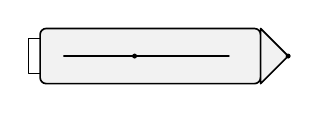
\begin{tikzpicture}[>=Latex, line cap=round, line join=round]

% ---------- styles (safe names) ----------
\tikzset{
  usvHull/.style   ={draw, line width=0.6pt, fill=gray!10},
  usvDetail/.style ={draw, line width=0.45pt},
  usvMark/.style   ={fill=black}
}

% ---------- USV: 2D top view ----------
% Main hull (rounded rectangle)
\path[usvHull, rounded corners=2.2pt]
  (-1.2,-0.35) rectangle (1.6,0.35);

% Bow wedge (forward direction)
\path[usvHull]
  (1.6,-0.35) -- (1.95,0) -- (1.6,0.35) -- cycle;

% Deck centerline (subtle)
\draw[usvDetail] (-0.9,0) -- (1.2,0);

% Reference anchors
\coordinate (usvCenter) at (0,0);
\coordinate (usvBow)    at (1.95,0);
\coordinate (usvStern)  at (-1.2,0);

% Anchor markers
\fill[usvMark] (usvCenter) circle (0.9pt);
\fill[usvMark] (usvBow)    circle (0.9pt);

% Stern notch (technical detail, still minimal)
\draw[usvDetail]
  (-1.2,-0.22) -- (-1.35,-0.22) -- (-1.35,0.22) -- (-1.2,0.22);

\end{tikzpicture}
\end{center}
\end{document}